%% LyX 2.3.1 created this file.  For more info, see http://www.lyx.org/.
%% Do not edit unless you really know what you are doing.
\documentclass[spanish]{article}
\usepackage[T1]{fontenc}
\usepackage[latin9]{inputenc}
\usepackage{geometry}
\geometry{verbose,tmargin=2cm,bmargin=2cm,lmargin=2cm,rmargin=2cm,headheight=2cm,headsep=2cm,footskip=2cm}
\usepackage{float}
\usepackage{graphicx}

\makeatletter

%%%%%%%%%%%%%%%%%%%%%%%%%%%%%% LyX specific LaTeX commands.
%% Because html converters don't know tabularnewline
\providecommand{\tabularnewline}{\\}

\makeatother

\usepackage{babel}
\addto\shorthandsspanish{\spanishdeactivate{~<>.}}

\begin{document}
\begin{titlepage}
\newcommand{\HRule}{\rule{\linewidth}{0.5mm}}       
\center        
%---------------------------------------------------------------------------------------- 
%	HEADING SECTIONS 
%----------------------------------------------------------------------------------------      
\textsc{\LARGE Instituto Tecnol�gico de Buenos Aires}\\[2cm]  
\textsc{\Large 22.42 Laboratorio de Electronica}\\[1.5cm]  
\textsc{\large Trabajo Pr�ctico de Laboratorio $N^o~5$ }\\[0.5cm]
%---------------------------------------------------------------------------------------- 
%	TITLE SECTION 
%----------------------------------------------------------------------------------------      
\HRule \\[0.5cm] 
{ \huge Analizador de Espectros  }
\\[0.4cm]  \HRule \\[2cm]       
%---------------------------------------------------------------------------------------- 
%	AUTHOR SECTION 
%----------------------------------------------------------------------------------------      
\begin{minipage}{0.4\textwidth} \begin{flushleft} \large 
\emph{Grupo 3:}\\		 [.3cm] 
Mat�as \textsc{Larroque}\\ Leg. 56597\\  [.3cm] 
Ariel \textsc{Martorell}\\ Leg. 56209\\  [.3cm] 
Manuel \textsc{Moll�n}\\ Leg. 58023 \\  [.3cm] 
Ezequiel \textsc{Vijande}\\ Leg. 58057\\  [.3cm] 
\end{flushleft} \end{minipage} ~ 
\begin{minipage}{0.4\textwidth} \begin{flushright} \large 
\emph{Profesor:} \\ [.3cm] 
Pablo Mart�n  \textsc{Cossutta}\\ 
Mar�a Alejandra  \textsc{Weill} \\ 
Mat�as Dami�n  \textsc{Salvati} 
\end{flushright} \end{minipage}\\[2cm]      
%---------------------------------------------------------------------------------------- 
%	DATE SECTION 
%----------------------------------------------------------------------------------------      
\vfill {\large Entregado: 20 de Noviembre de 2018}\\[2cm]      \vfill       
\end{titlepage}

\pagebreak{}

\tableofcontents{}

\pagebreak{}

\section{Introducci�n}

En este escrito se busca exponer algunas de las distintas aplicaciones
de un analizador de espectros. Asimismo, se dar�n algunas descripciones
breves de conceptos relacionados con el estudio de las se�ales en
el dominio de la frecuencia y la utilidad de los mismos. Con este
fin, se muestran un numero de mediciones realizadas con dicho instrumento
y en lo posible la simulacion teorica del fenomeno de inter�s.

\section{Total Harmonic Distortion(THD)}

La distorsion armonica es un concepto que hace referenca a que tan
'impura' es una senal, ya que establece una relacion entre la ampliud
de los armonicos secundarios de la senal con el armonico fundamental.
La defincion matematica de la misma es:
\begin{center}
\begin{equation}
THD=\frac{\sum_{i=1}^{\infty}P_{i}}{P_{0}}
\end{equation}
\par\end{center}

Donde $P_{i}$ representa la potencia de los armonicos secundarios
de la senal y $P_{0}$ es la potencia del armonico fundamental. En
la practica no es posible hacer la suma de los infinitos armonicos
por lo que en este trabajo medimos todos los armonicos detectados
por el instrumento (aquellos con potencia mayor a -80dbm).

Se conectaron 3 generadores de senales distintos al analizador de
espectros,aunque todos del mismo modelo(Agilent 33220A, 20MHz), y
se procedio a medir la potencia de todos los armonicos presentes con
el fin de calcular la THD de cada uno.

Dicha medicion se llevo a cabo para una senal senoidal de una amplitud
de 250mVpp y una frecuencia fundamental de 900KHz.A continuacion se
presenta una tabla con los resultados obtenidos:
\begin{center}
\begin{table}
\begin{centering}
\begin{tabular}{|c|c|c|c|c|c|c|}
\hline 
 & $P_{0}$(dbm) & $P_{1}$(dbm) & $P_{2}$(dbm) & THD(medido) & Error & THD(manual)\tabularnewline
\hline 
\hline 
$1^{er}$Generador & -43 & - & -77 & 0.04\% &  & 0.04\%\tabularnewline
\hline 
$2^{do}$Generador & -45 & - & -75.2 & 0.01\% &  & 0.04\%\tabularnewline
\hline 
$3^{er}$Generador & -35 & - & -70 & 0.03\% &  & 0.04\%\tabularnewline
\hline 
\end{tabular}
\par\end{centering}
\caption{THD medida de cada generador}
\end{table}
\par\end{center}

Las mediciones anteriores se realizaron centrando la pantalla en la
frecuencia de cada armonico con un Span de 100KHz y un RBW de 1Khz.

\section{Espectros de distintas se�ales}

Se procedio a realizar la medicion del espectro de distintas formas
de onda, todas de 250mVpp y de una frecuencia fundamental de 900KHz.

\subsection{Senal cuadrada}

\subsection{Senal triangular}

\subsection{Tren de pulsos}

\section{Modulacion AM y FM}

Mediante el uso de dos generadores se procedio a generar una senal
modulada en AM de 200mVpp. Se utilizo un generador de ondas para producir
la senal correspondiente a la moduladora(se utilizo $f_{m}=100KHz$)
y el otro para producir la senal de la portadora($f_{p}=1.1MHz$).
Luego se repitio la experiencia con las dos ondas de las mismas caracteristicas
pero con el objetivo de producir una senal modulada en FM.

\subsection{Resultados AM}

A continuacion se presentan imagenes obtenidas del analizador de espectros
para distintos casos de interes, acompanados por su correspondiente
simulacion.
\begin{itemize}
\item Moduladora senoidal, m=0.5
\end{itemize}
\begin{center}
\begin{figure}[H]
\begin{centering}
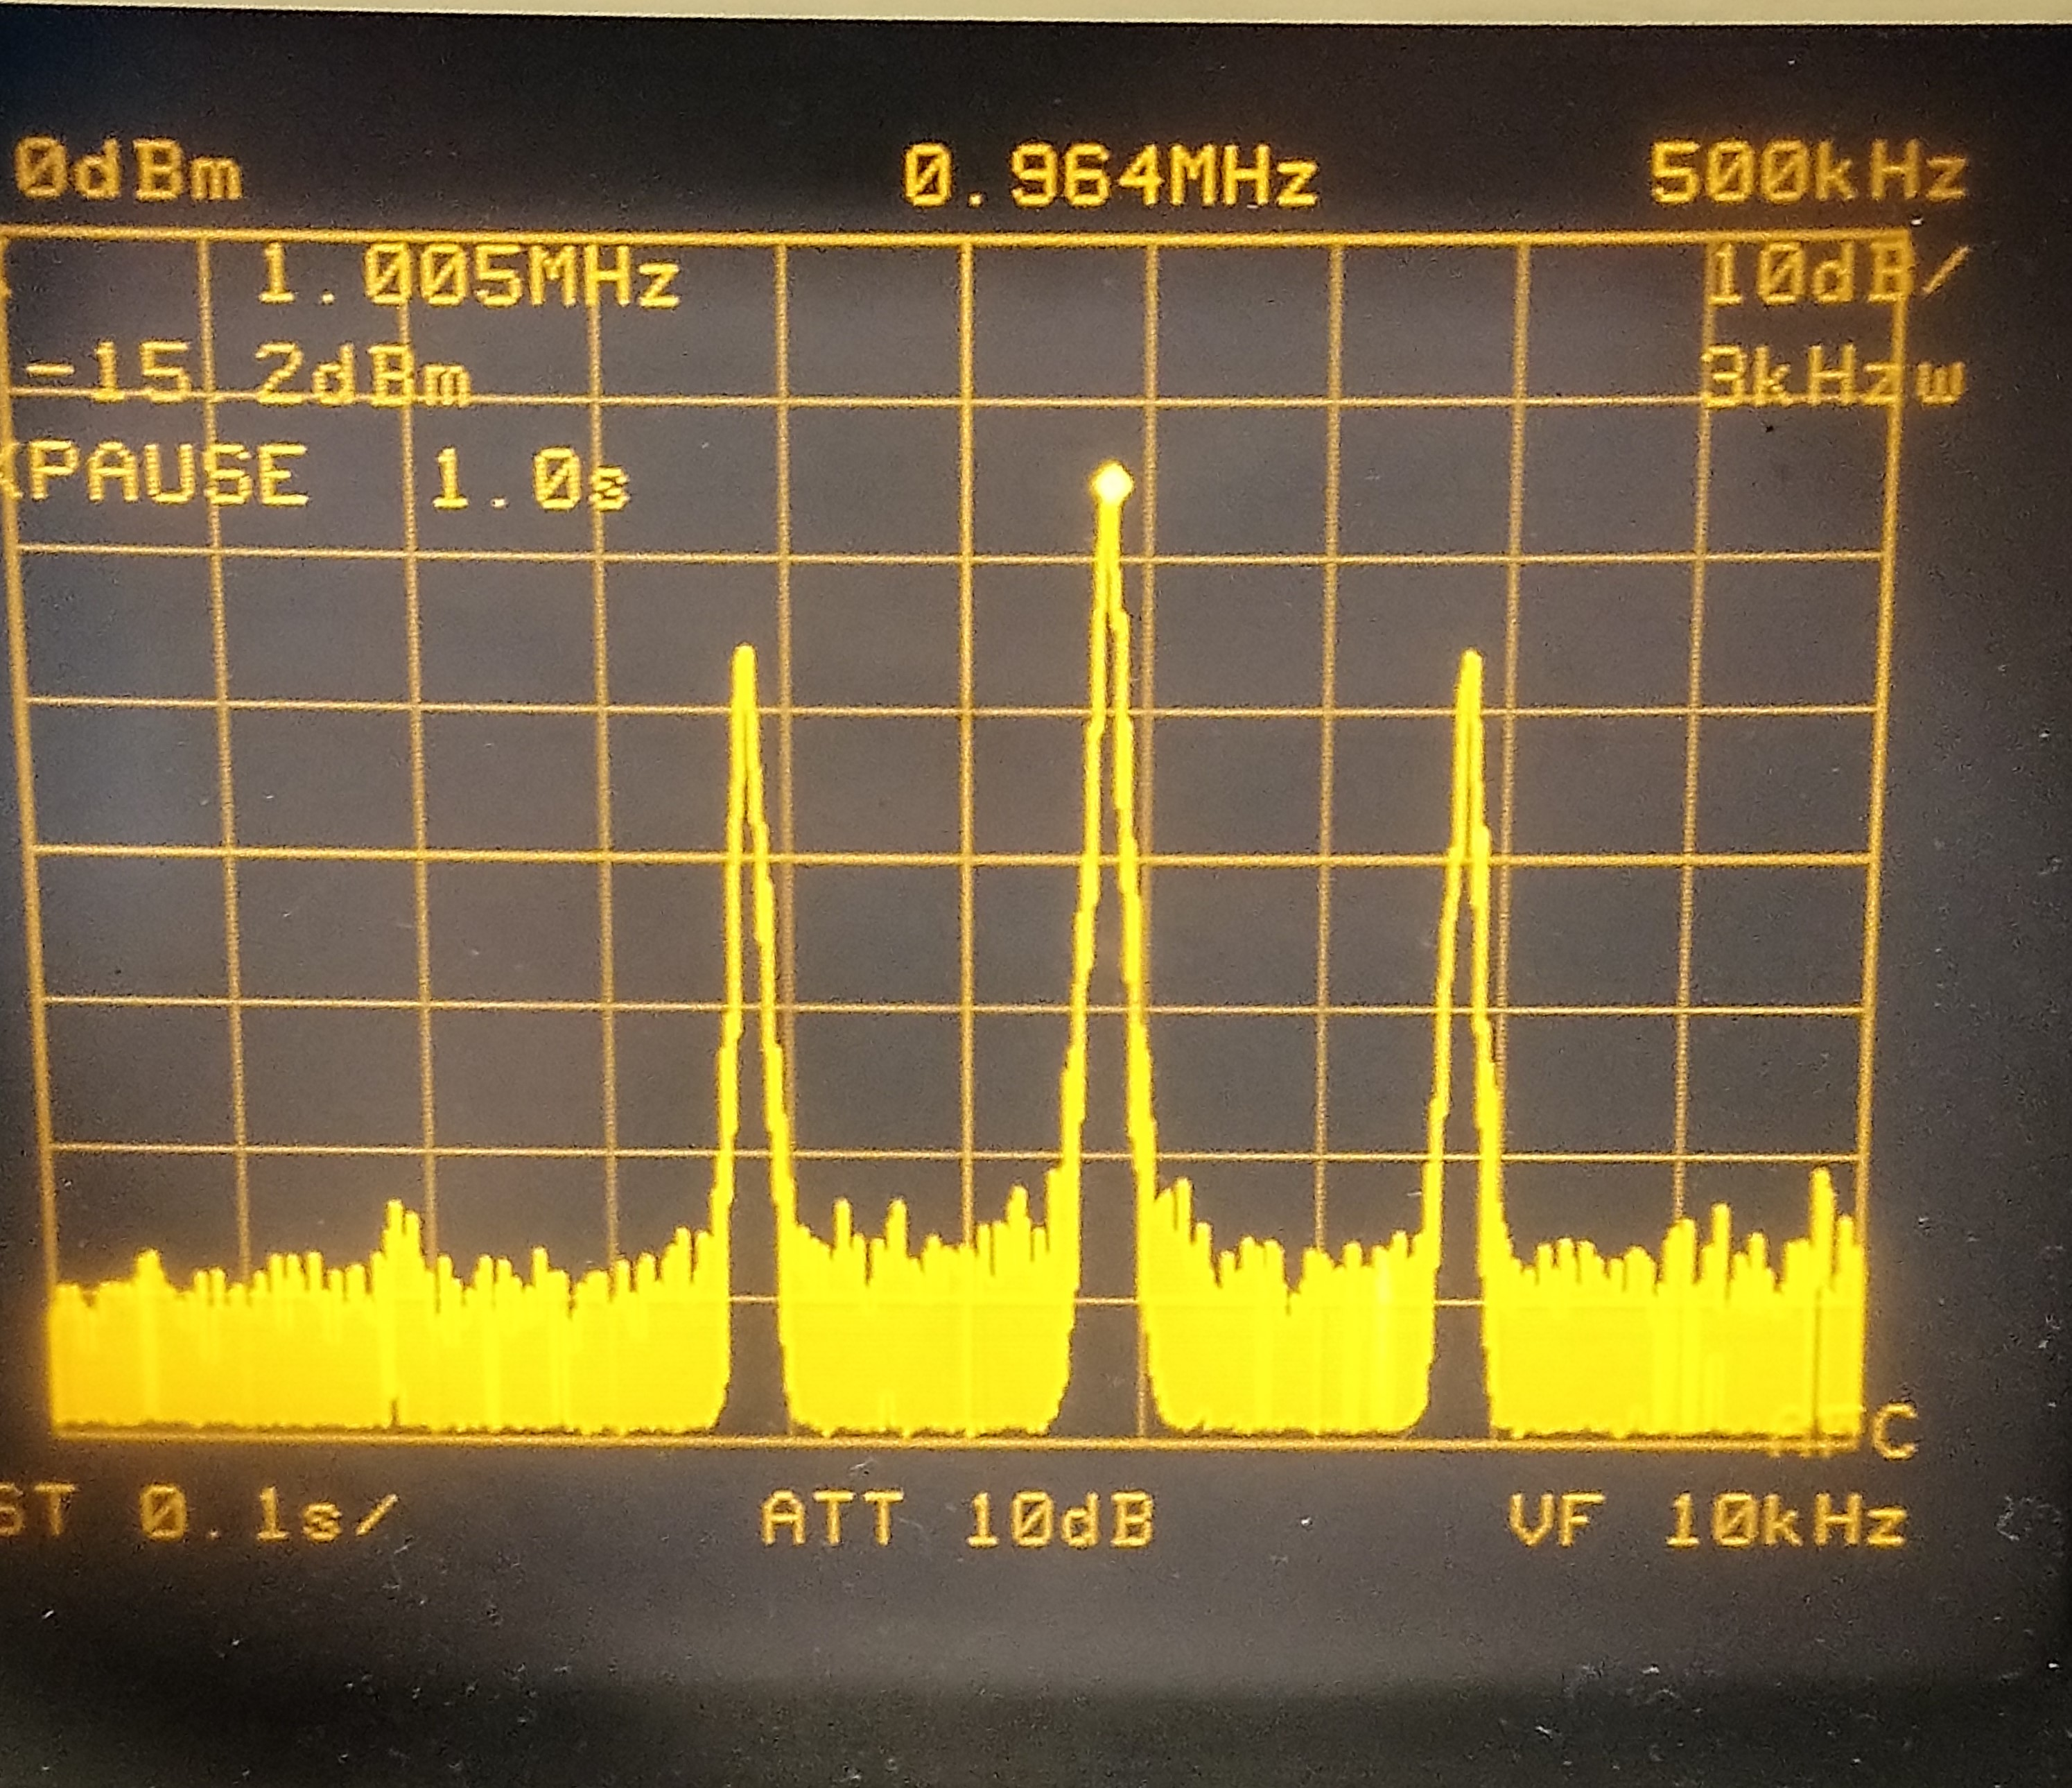
\includegraphics[scale=0.25]{Imagenes/DSC_0044.JPG}
\par\end{centering}
\caption{Medicion para m=0.5}

\end{figure}
\par\end{center}
\begin{itemize}
\item Moduladora senoidal, m=1
\end{itemize}
\begin{center}
\begin{figure}[H]
\begin{centering}
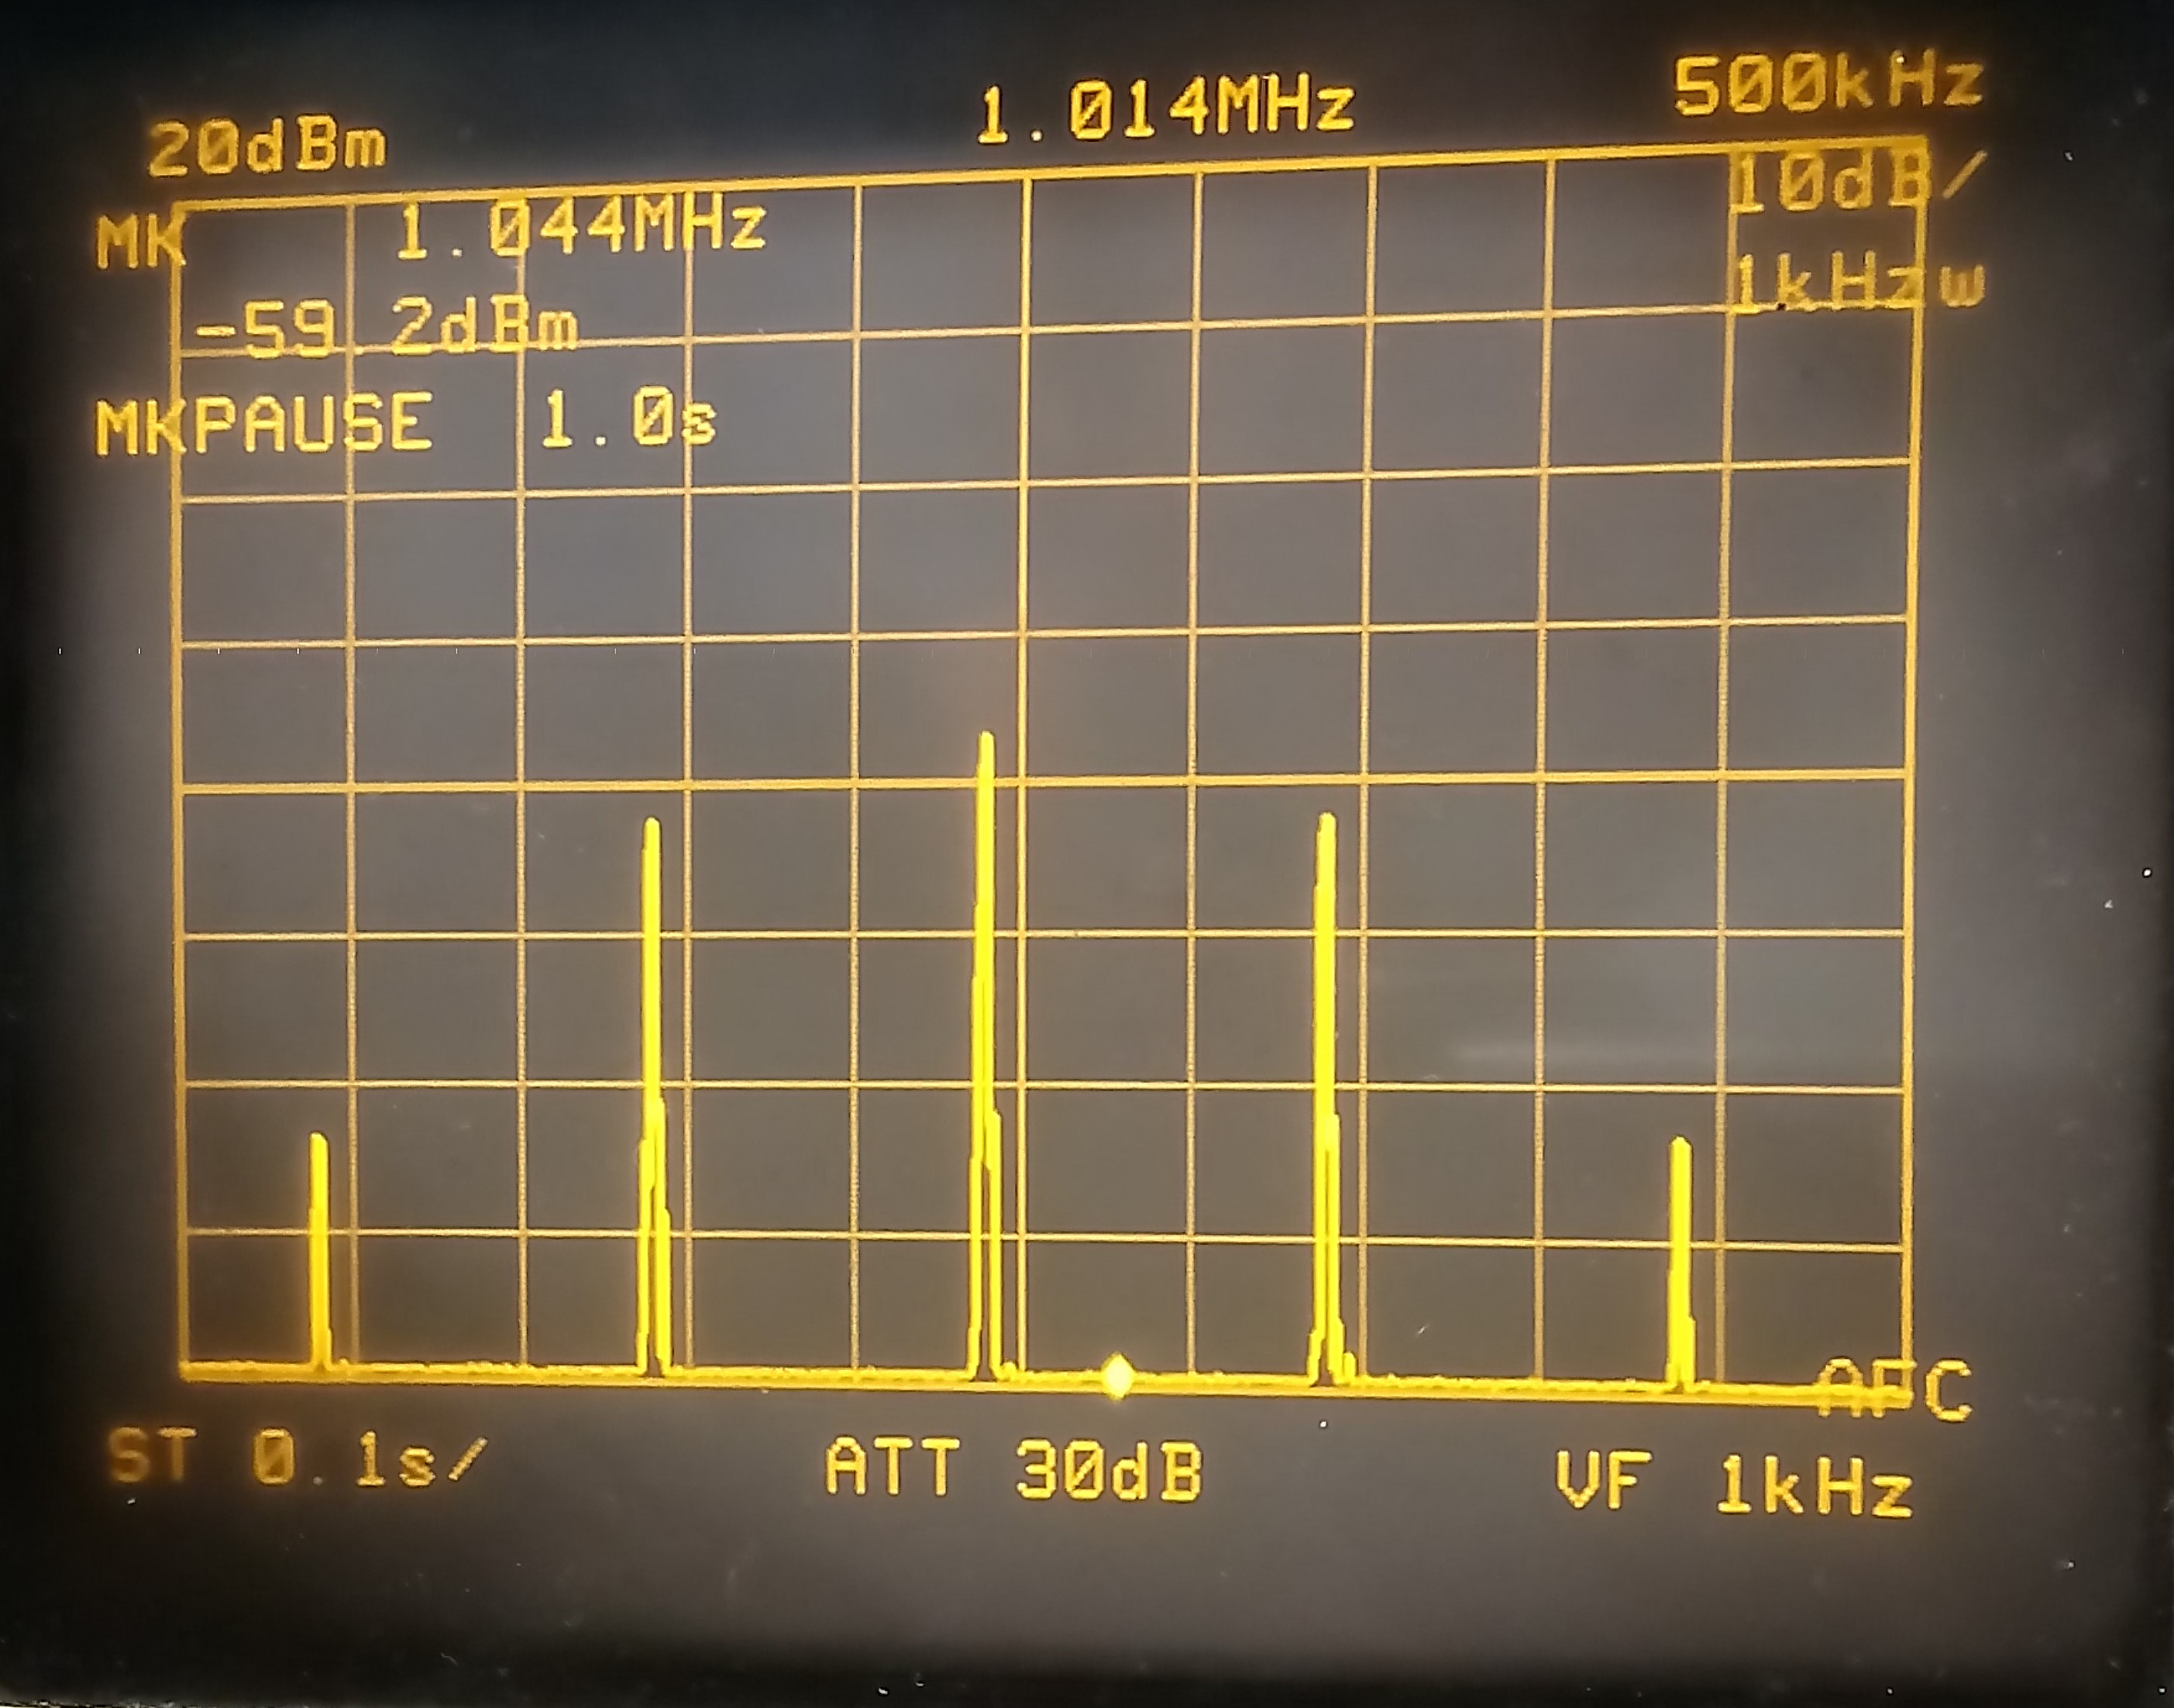
\includegraphics[scale=0.25]{Imagenes/DSC_0045.JPG}
\par\end{centering}
\caption{Medicion obtenida para m=1}

\end{figure}
\par\end{center}
\begin{itemize}
\item Moduladora triangular, m=1
\end{itemize}
\begin{center}
\begin{figure}[H]
\begin{centering}
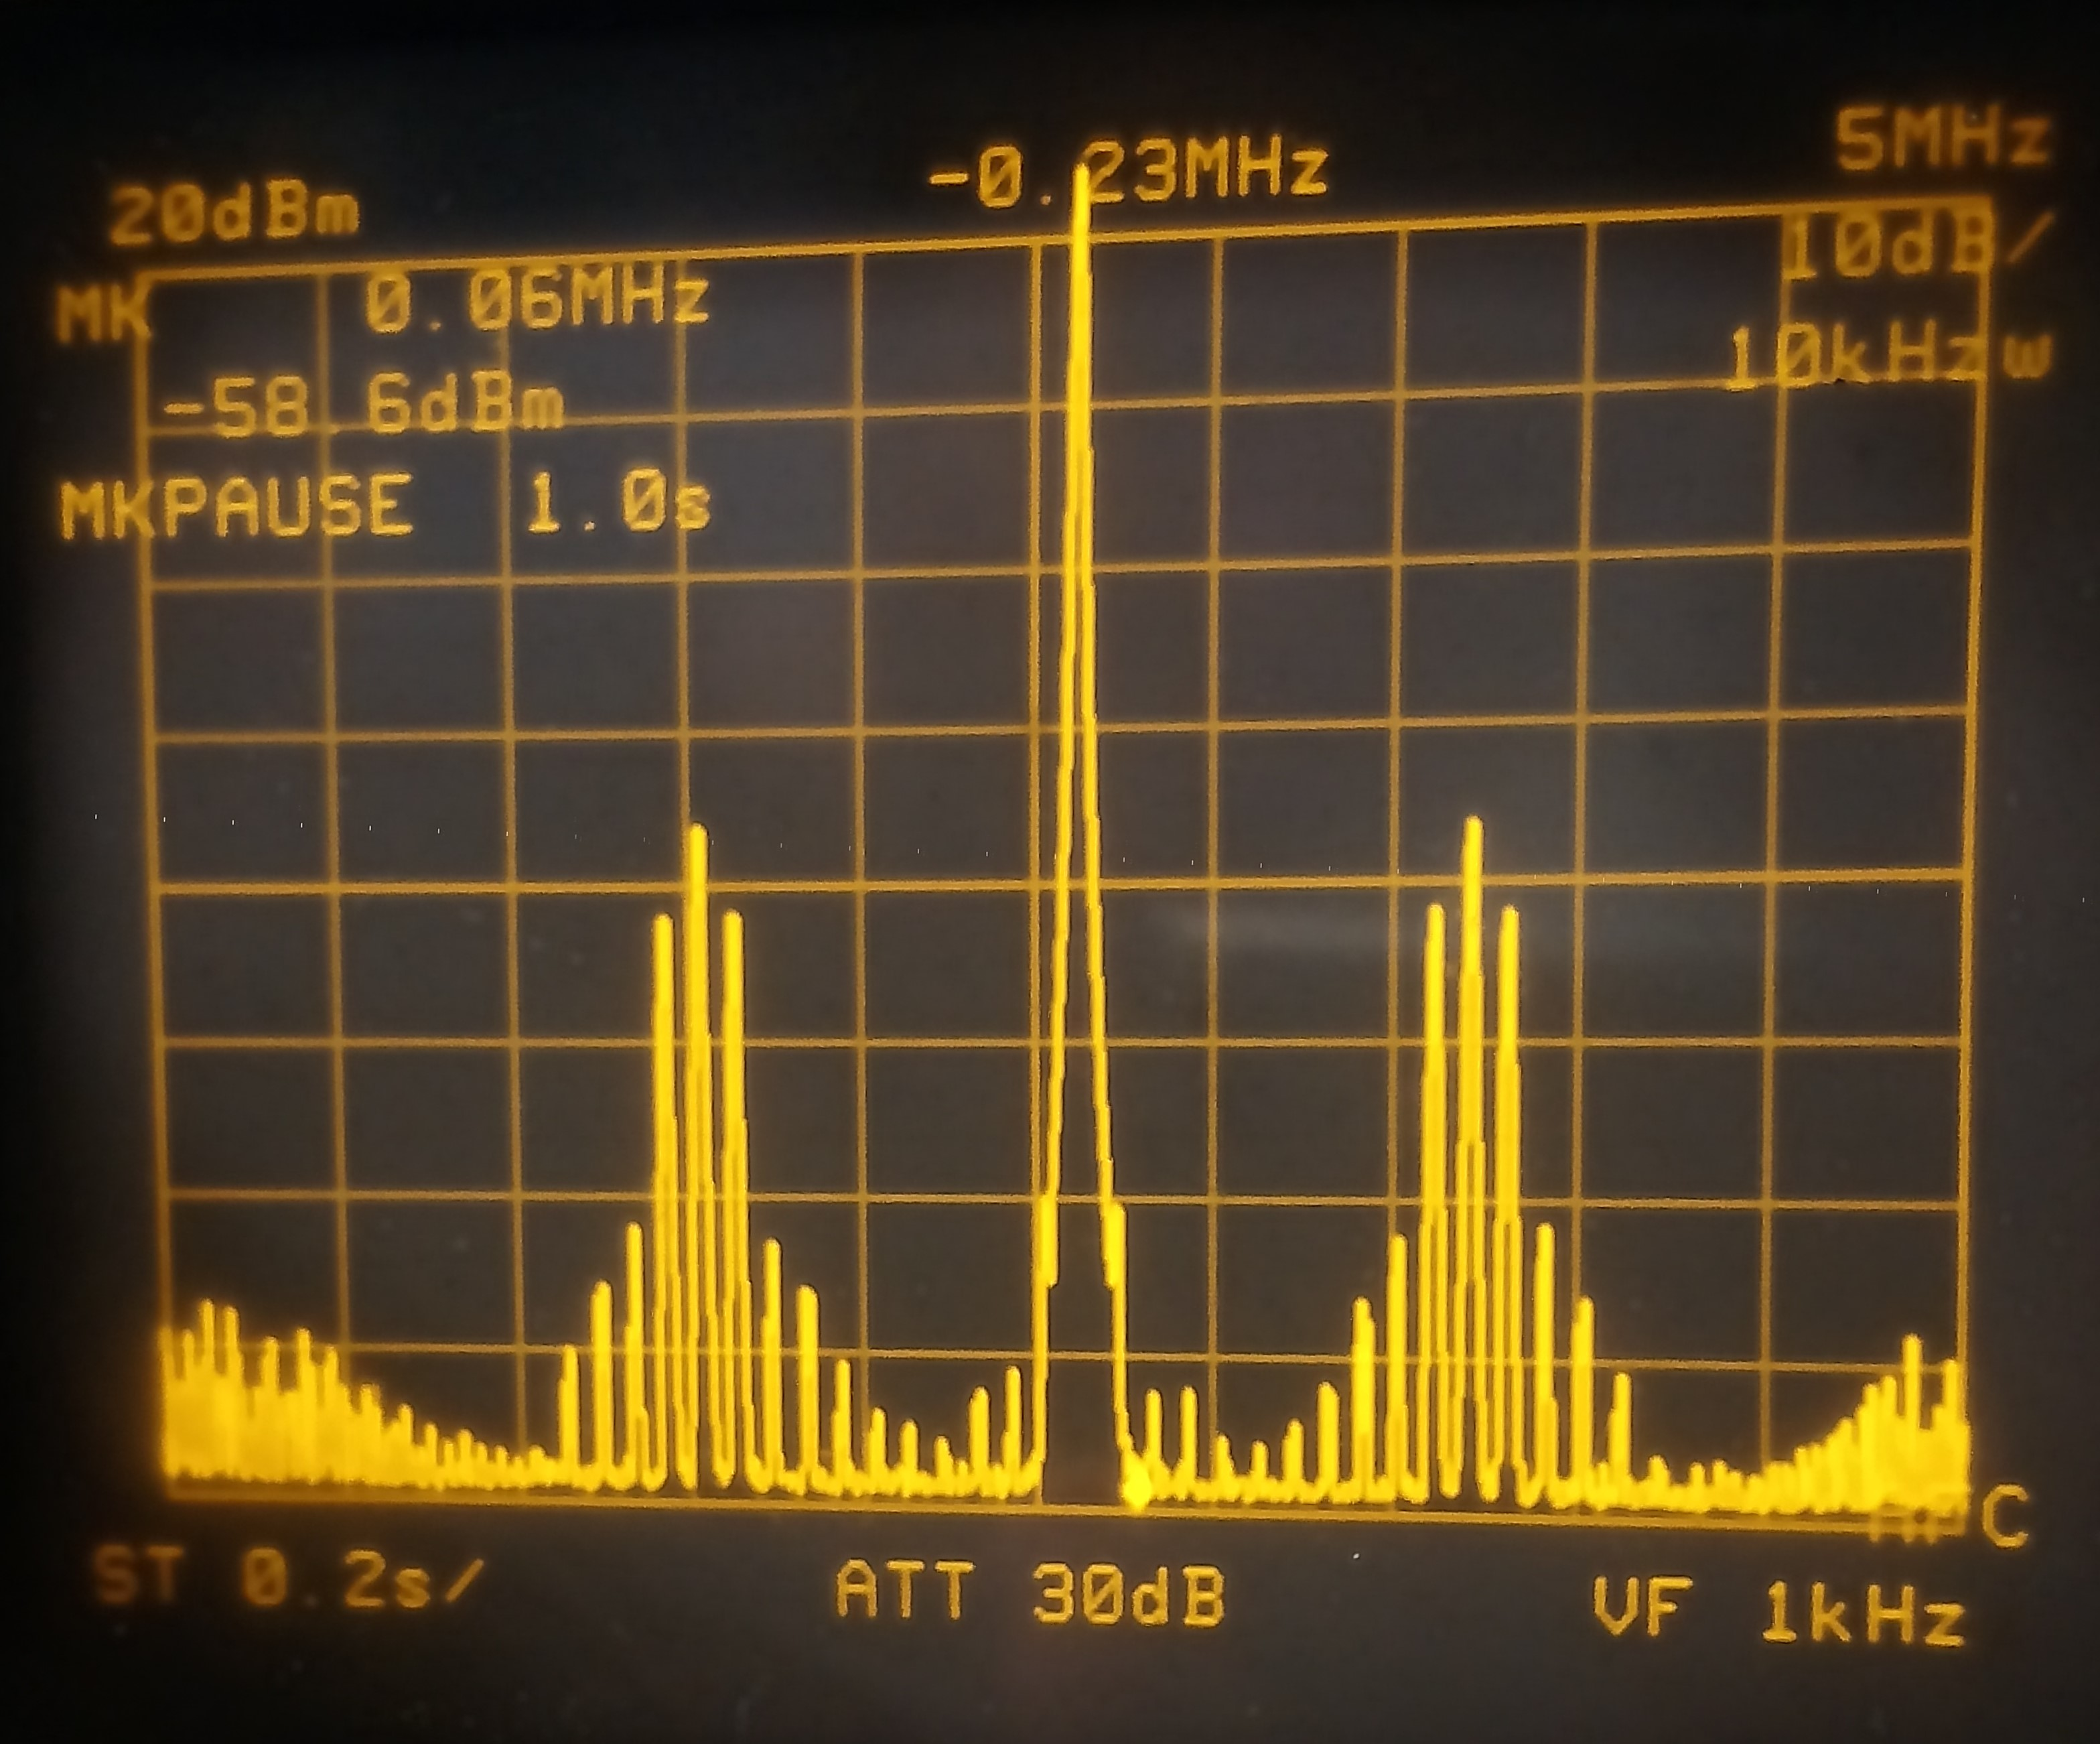
\includegraphics[scale=0.25]{Imagenes/DSC_0046.JPG}
\par\end{centering}
\caption{Medicion para moduladora triangular y m=1}

\end{figure}
\par\end{center}
\begin{itemize}
\item Moduladora senoidal,m=1 ($f_{m}=1.1MHz$)
\end{itemize}
\begin{center}
\begin{figure}[H]
\begin{centering}
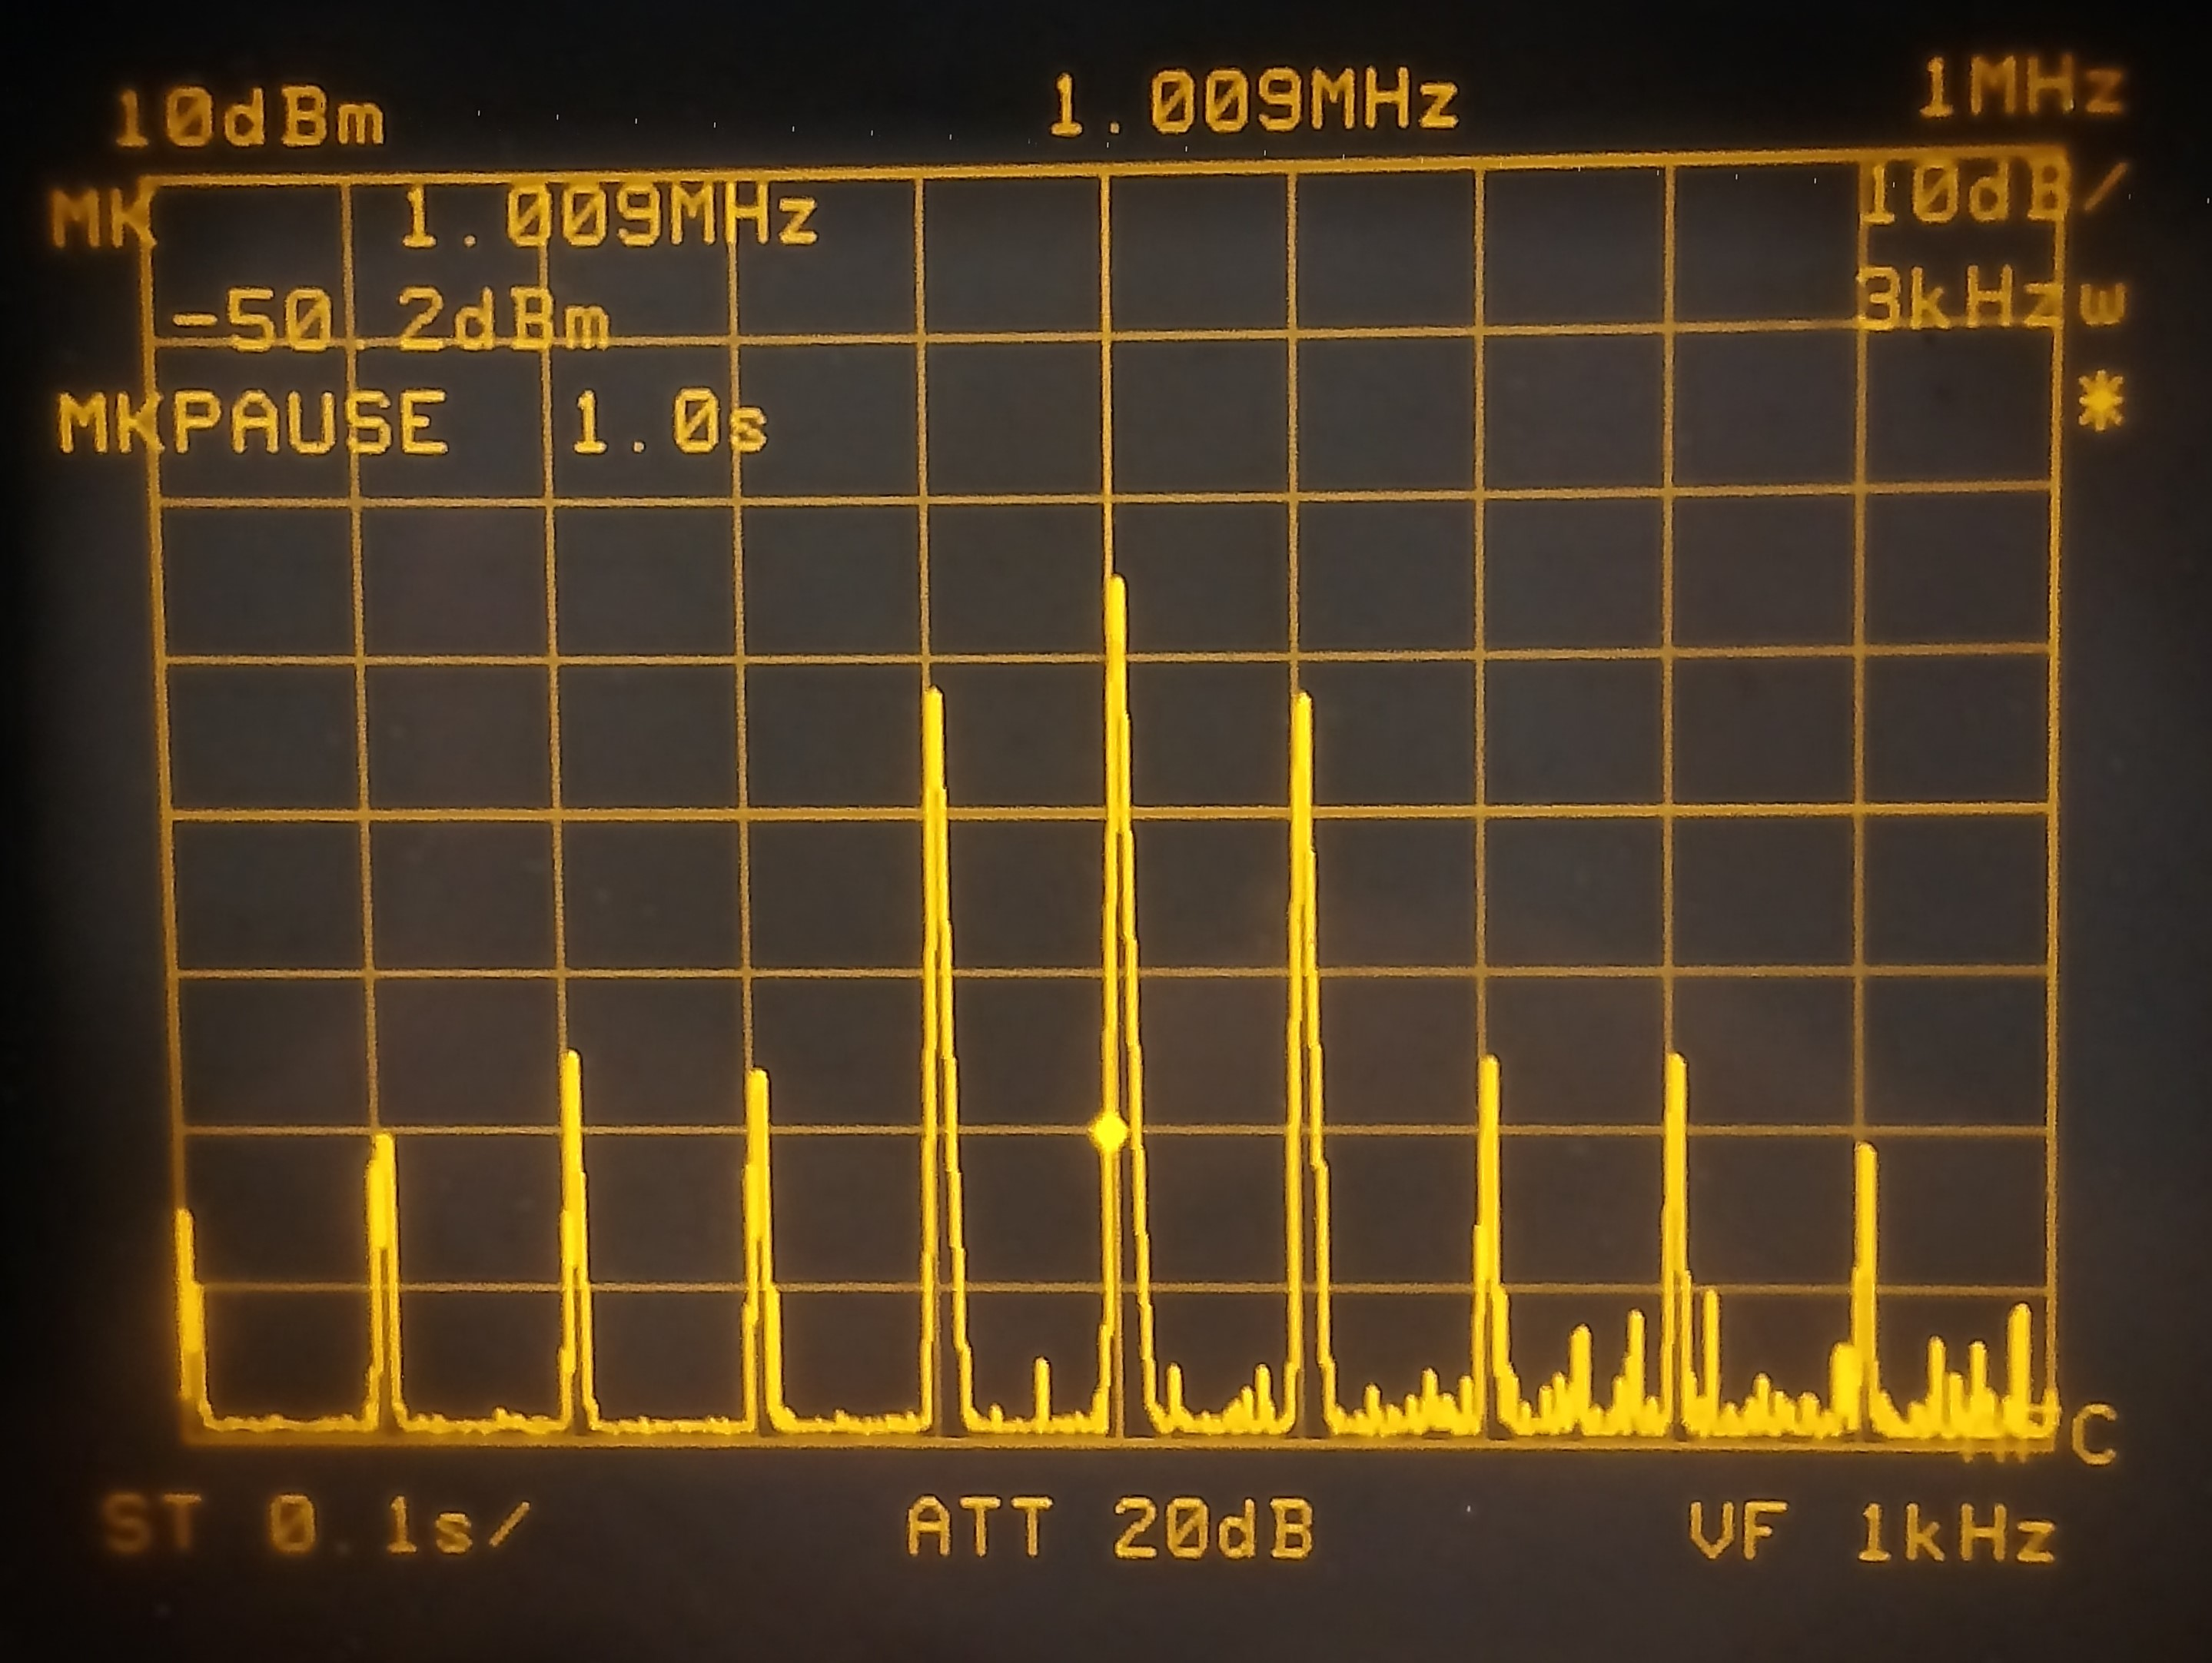
\includegraphics[scale=0.25]{Imagenes/DSC_0048.JPG}
\par\end{centering}
\caption{Medicion para m=1 y $f_{m}=f_{p}=1.1MHz$}

\end{figure}
\par\end{center}

\subsection{Resultados FM}
\begin{itemize}
\item Moduladora senoidal, m=0.5
\end{itemize}
\begin{center}
\begin{figure}[H]
\caption{Medicion para m=0.5}
\end{figure}
\par\end{center}
\begin{itemize}
\item Moduladora senoidal, m=1
\end{itemize}
\begin{center}
\begin{figure}[H]
\caption{Medicion obtenida para m=1}
\end{figure}
\par\end{center}
\begin{itemize}
\item Moduladora triangular, m=1
\end{itemize}
\begin{center}
\begin{figure}[H]
\caption{Medicion para moduladora triangular y m=1}
\end{figure}
\par\end{center}
\begin{itemize}
\item Moduladora senoidal,m=1 ($f_{m}=1.1MHz$)
\end{itemize}
\begin{center}
\begin{figure}[H]
\caption{Medicion para m=1 y $f_{m}=f_{p}=1.1MHz$}
\end{figure}
\par\end{center}

\section{Espectro de radiofrecuencias en Argentina}

A continucaci�n se procede a realizar un estudio del espectro de radiorecuencias
en Argentina, por lo cual en el siguiente cuadro se procede a mostrar
las frecuencias de operaci�n y los niveles de potencia que emiten
los diversos sistemas y servicios de comunicai�n que utilizan radiofrecuencias:

\begin{table}
\begin{centering}
\includegraphics[scale=0.45]{\string"Imagenes/atribucci�n espectro de radiofrecuencias\string".JPG}\caption{Distribuci�n de Radiofrecuencia\label{tab:Distribuci=0000F3n-de-Radiofrecuencia}}
\par\end{centering}
\end{table}

\subsection{Medici�n se�ales de telefon�a celular - $878\,MHz$}

Como se puede observar en el cuadro (\ref{tab:Distribuci=0000F3n-de-Radiofrecuencia})
esta frecuencia pertenece al rango de servicios de telefon�a m�vil,
dichas se�ales presentan un sonido pero no es uno que brinde demasiada
informaci�n pero que se pod�a diferenciar considerablemente del sonido
del ruido el�ctrico que produce el analizador.

En esta frecuencia se obtuvo considerando un $ span=100\,MHz $ y
un $ RBW=1\,MHz $ con el que se obtuvo una medici�n de potencia de
$ P=-57\,dBm. $ 

\section{Espectro de FM}

Para este ejercicio se prodcedio a analizar el espectro electromagnetico
en la banda FM, elegir una emisora, sintonizarla utilizando el analizador
de espectros y obtener su potencia.

\subsection{Medici�n }

En esta medici�n se sintonizo una frecuencia correspondiente a una
radio en este caso a radio La Plata cuya frecuencia es de $92.1\,MHz$,
una vez que se pudo sintonizar dicha estaci�n y verificar que era
la misma escuchando su contenido, se procedio a medir su potencia
y se obtuvo que $P=-40\,dBm$

\section{Espectro de televisi�n}

El espectro de radiofrecuencia de la televisi�n argentina esta dividido
en 3 bandas como se muestra en la siguiente tabla:

\begin{table}
\centering{}%
\begin{tabular}{|c|c|}
\hline 
Banda & Frecuencias {[}Mhz{]}\tabularnewline
\hline 
\hline 
VHF Bajo & $54-88$\tabularnewline
\hline 
VHF alto & $174-216$\tabularnewline
\hline 
UHF & $512-806$\tabularnewline
\hline 
\end{tabular}\caption{Distribucio�n de las bandas de televisi�n}
\end{table}

\subsection{Medici�n }

Para esta medici�n se busco sintonizar la frecuencia correspondiente
al canal 13 de aire que se obtuvo a la frecuencia $ f=215,7\,Mhz $
con el cual utilizando un $span=500\,kHz$ y un $ RBW= 100\,Khz $
se obtuvo la siguienta potencia a partir de la medici�n $P=-37.6\,dBm $.
En dicha medici�n se pudo escuchar claramente el sonido emitido por
el programa de televisi�n que estaba siendo emitido en el instante
de la medici�n.

\section{$\frac{Sin(x)}{x}$ y Tren de deltas}

Para realizar el siguiente ejercicio se utiliz� un generador de se�ales
que pose�a ya tanto el $sinc(x)$ como el tren de ddeltas previamente
cargadas, con las que se obtuvieron las siguientes mediciones.

\begin{figure}
\caption{Espectro del $sinc(x)$\label{fig:Espectro-del}}
\end{figure}
\begin{figure}
\caption{Espectro del tren de deltas\label{fig:Espectro-del-tren}}
\end{figure}
Como se puede observar en ambas figuras (\ref{fig:Espectro-del})
y (\ref{fig:Espectro-del-tren}) se puede observar claramente sus
respectivas transformadas de Fourier.

\section{Conclusiones}

Para Finalizar, se pudo contemplar la funcionalidad que posee el analizador,
que nos posibilit� el sintonizar radiofrecuencias y a su vez medir
sus espectros tanto como medir el espectro de distintas se�ales, consecuentemente
se pudo comprobar que dichas mediciones coinciden con el c�lculo te�rico
del espectro de las se�ales medidas que se obtuvo mediante la transformada
de Fourier.

\pagebreak
\end{document}
